% Uncomment this line for on-screen presentation
\documentclass[xcolor={dvipsnames}]{beamer}\usepackage{etoolbox}\newtoggle{printable}\togglefalse{printable}

% Uncomment this line for printable slides (disable animations and don't waste ink)
%\documentclass[handout, xcolor={dvipsnames}]{beamer}\usepackage{etoolbox}\newtoggle{printable}\toggletrue{printable}

% Adjust these for the path of the theme and its graphics, relative to this file
%\usepackage{beamerthemeFalmouthGamesAcademy}
\usepackage{../../beamerthemeFalmouthGamesAcademy}
\graphicspath{ {../../} }

% Default language for code listings
\lstset{language=C++,
		morekeywords={each,in}
}

\begin{document}
\title{Transition to C++ II}   
\subtitle{COMP110: Principles of Computing}

\frame{\titlepage} 

\begin{frame}{Learning outcomes}
	In this session you will learn how to...
	\begin{itemize}
		\item Split your program into multiple files, and understand the difference between
		    \textbf{source files} and \textbf{header files}
		\item Understand the C++ build pipeline, and the roles of the \textbf{preprocessor},
		    \textbf{compiler} and \textbf{linker}
		\item Use arrays, and the difference between creating them on the \textbf{stack}
		    versus on the \textbf{heap}
		\item Define C++ functions, and how passing \textbf{by reference} differs from passing \textbf{by value}
	\end{itemize}
\end{frame}

\part{Modular program design}
\frame{\partpage}

\begin{frame}{Modular program design}
	\begin{itemize}
		\pause\item Writing a piece of software as a
			\textbf{single long source file} is generally a bad idea
		\pause\item Better to split the program into several self-contained files,
			i.e.\ \textbf{modules}
		\pause\item Makes code easier to \textbf{navigate}
		\pause\item Allows related classes and functions to be
			\textbf{grouped} together
		\pause\item Modules can often be \textbf{reused} between programs
		\pause\item In compiled languages, can allow for faster iteration via
			\textbf{incremental recompilation}
	\end{itemize}
\end{frame}

\begin{frame}[fragile]{Modules in Python}
	\begin{itemize}
		\pause\item \textbf{Every} Python source file is a \textbf{module}
		\pause\item Can be loaded using the \lstinline{import} statement,
			just like built-in modules
	\end{itemize}
	\begin{columns}
		\begin{column}{0.48\textwidth}
			\pause mymodule.py
			\begin{lstlisting}
def test():
    print "Hello world!"
			\end{lstlisting}
		\end{column}
		\begin{column}{0.48\textwidth}
			\pause program.py
			\begin{lstlisting}
import mymodule

mymodule.test()
			\end{lstlisting}
		\end{column}
	\end{columns}
\end{frame}

\begin{frame}[fragile]{Modules vs programs}
	\begin{itemize}
		\pause\item How to tell if a Python file is a program or a module?
		\pause\item Every Python file can be used as both, but you can check
			at runtime:
	\end{itemize}
	\begin{lstlisting}
if __name__ == "__main__":
    print "I am a program"
else:
    print "I am an imported module"
	\end{lstlisting}
	\begin{itemize}
		\pause\item \lstinline{__name__} is a built-in variable (note the
			double underscores!)
	\end{itemize}
\end{frame}


\part{The build process}
\frame{\partpage}

\begin{frame}{Executing programs}
    \begin{itemize}
        \item CPUs execute \textbf{machine code}
        \item Programs must be \textbf{translated} into machine code for execution
        \item There are three main ways of doing this:
        \begin{itemize}
            \item An \textbf{interpreter} is an application which reads the program source code and executes it directly
            \item A \textbf{compiler} is an application which converts the program source code into executable machine code
            \item A \textbf{just-in-time (JIT) compiler} is halfway between the two --- it compiles the program on-the-fly
                at runtime
        \end{itemize}
    \end{itemize}
\end{frame}

\begin{frame}{Examples}
	\begin{columns}[t,onlytextwidth]
		\begin{column}{0.3\textwidth}
		    Interpreted:
		    \begin{itemize}
		        \item Python
		        \item Lua
		        \item Bespoke scripting languages
		    \end{itemize}
		\end{column}
		\begin{column}{0.3\textwidth}
		    Compiled:
		    \begin{itemize}
		        \item C
		        \item C++
		        \item Swift
		    \end{itemize}
		\end{column}
		\begin{column}{0.3\textwidth}
		    JIT compiled:
		    \begin{itemize}
		        \item Java
		        \item C\#
		        \item JavaScript (in modern web browsers)
		        \item Jython
		    \end{itemize}
		\end{column}
	\end{columns}
\end{frame}

\begin{frame}{Interpreter vs compiler}
    \begin{itemize}
        \item Run-time efficiency: compiler $>$ interpreter
        \begin{itemize}
            \item The compiler translates the program \textbf{in advance}, on the developer's machine
            \item The interpreter translates the program \textbf{at runtime}, on the user's machine
        \end{itemize}
        \item Portability: compiler $<$ interpreter
        \begin{itemize}
            \item A compiled program can only run on the operating system and CPU architecture it was compiled for
            \item An interpreted program can run on any machine, as long as a suitable interpreter is available
        \end{itemize}
        \item For games, run-time efficiency is usually much more important than portability
    \end{itemize}
\end{frame}

\begin{frame}[fragile]{The C++ build process}
    \textbf{Preprocessor}
    \begin{itemize}
        \item Replaces \lstinline{#include} directives with the contents of the appropriate header files
        \item Handles other preprocessor directives (\lstinline{#define}, \lstinline{#if} etc --- more on these another time)
    \end{itemize}
    \textbf{Compiler}
    \begin{itemize}
        \item Translates each source file into an \textbf{object file} containing machine code
    \end{itemize}
    \textbf{Linker}
    \begin{itemize}
        \item Combines the object files together with any external libraries to produce an \textbf{executable}
            (on Windows, a .exe file)
    \end{itemize}
\end{frame}

\begin{frame}[fragile]{The C++ build process}
    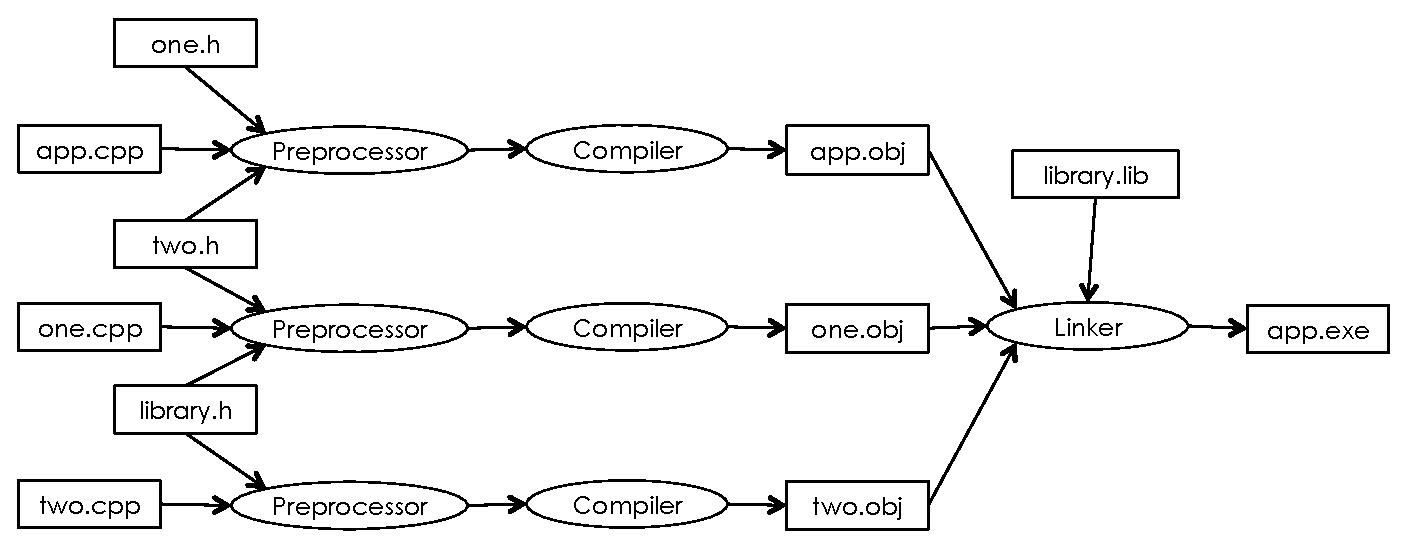
\includegraphics[width=\textwidth]{compiler_flowchart.pdf}
\end{frame}

\begin{frame}[fragile]{Incremental compilation}
    \begin{itemize}
        \item Compilation takes time --- compiling a AAA game can take several hours
        \item Visual C++ stores intermediate files (e.g.\ \texttt{.obj} files) on disk
        \item Only the changed files need to be run through the preprocessor and compiler again
            $\implies$ faster re-compilation during development
        \item \textbf{Build $\to$ Clean} removes all intermediate files
        \item \textbf{Build $\to$ Rebuild} forces Visual C++ to recompile everything
    \end{itemize}
\end{frame}

\begin{frame}[fragile]{Precompiled headers}
    \begin{itemize}
        \item Headers may need to be compiled multiple times if they are included in multiple source files
        \item Headers may be very large ---
            e.g.\ \texttt{Windows.h} includes dozens of headers totalling many thousands of lines
        \item In Visual C++ projects, \texttt{stdafx.h} is a \textbf{precompiled header}
        \item \lstinline{#include "stdafx.h"} doesn't work like copy and paste ---
            instead, the compiler uses the precompiled header information
        \item Precompiled header only needs to be recompiled if \texttt{stdafx.h} (or something it includes)
            changes, which should be rare
    \end{itemize}
\end{frame}

\begin{frame}[fragile]{Build configuration in VC++}
    \begin{center}
        \includegraphics[width=0.6\textwidth]{vcpp_build_toolbar.PNG}
    \end{center}
    \begin{itemize}
        \item Configuration:
        \begin{itemize}
            \item \textbf{Debug} allows use of the Visual C++ debugger
            \item \textbf{Release} produces optimised code --- usually 2--10 $\times$ faster than Debug
            \item Generally use Debug for development, Release for optimisation and distributing the finished application
        \end{itemize}
        \item Platform:
        \begin{itemize}
            \item \textbf{x86} runs on 32-bit and 64-bit versions of Windows
            \item \textbf{x64} runs on 64-bit Windows only
            \item Generally use x86 for maximum compatibility, x64 for apps which need to use $>2$GB memory
                or where a significant speed benefit is measured
        \end{itemize}
    \end{itemize}
\end{frame}

\part{Arrays and lists}
\frame{\partpage}

\begin{frame}{Memory allocation --- recap}
	\begin{itemize}
		\pause\item Memory is allocated in \textbf{blocks}
		\pause\item The program specifies the size, in bytes, of the block it wants
		\pause\item The OS allocates a \textbf{contiguous} block of that size
		\pause\item The program owns that block until it frees it
		\pause\item Blocks can be allocated and deallocated at will, but can \textbf{never grow or shrink}
	\end{itemize}
\end{frame}

\begin{frame}{Collection types}
	\begin{itemize}
		\pause\item Memory management is hard and programmers are lazy
		\pause\item Collections are an \textbf{abstraction}
			\begin{itemize}
				\pause\item Hide the details of memory allocation, and allow the programmer to write simpler code
			\end{itemize}
		\pause\item Collections are an \textbf{encapsulation}
			\begin{itemize}
				\pause\item Bundle together the data's representation in memory along with the algorithms for accessing it
			\end{itemize}
	\end{itemize}
\end{frame}

\begin{frame}{Arrays}
	\begin{itemize}
		\pause\item An \textbf{array} is a contiguous block of memory in which objects are stored,
			equally spaced, one after the other
		\pause\item Each array element has an \textbf{index}, starting from zero
		\pause\item Given the address of the $0$th element, it is easy to find the $i$th element:
	\end{itemize}
	$$ \text{address}_i = \text{address}_0 + (i \times \text{elementSize}) $$
	\begin{itemize}
		\pause\item E.g.\ if the array starts at address $1000$ and each element is $4$ bytes,
			the 3rd element is at address $1000 + 4 \times 3 = 1012$
		\pause\item Accessing an array element is \textbf{constant time} $O(1)$
	\end{itemize}
\end{frame}

\begin{frame}{Lists}
	\begin{itemize}
		\pause\item An array is a block of memory, so its size is \textbf{fixed} once created
		\pause\item A \textbf{list} is a variable size array
		\pause\item When the list needs to change size, it \textbf{creates} a new array,
			\textbf{copies} the contents of the old array, and \textbf{deletes} the old array
	\end{itemize}
\end{frame}

\begin{frame}[fragile]{Arrays and lists in C\#}
	\begin{lstlisting}
int[] myArray = new int[10];

int[] myOtherArray = new int[] { 2, 3, 5, 7, 11 };

List<int> myList = new List<int>();

List<int> myOtherList = new List<int> { 2, 3, 5, 8, 13 };
	\end{lstlisting}
\end{frame}

\begin{frame}{Time taken to append an element to a list of size $n$}
	\begin{center}
		\vspace{-5ex}
		\includegraphics[height=0.9\textheight]{list_append_timing}
	\end{center}
\end{frame}

\begin{frame}{Operations on lists}
	\begin{itemize}
		\pause\item \textbf{Appending} to a list is \textbf{amortised constant time}
			\begin{itemize}
				\pause\item Usually $O(1)$, but can go up to $O(n)$ if the list needs to change size
			\end{itemize}
		\pause\item \textbf{Inserting} anywhere other than the end is \textbf{linear time}
			\begin{itemize}
				\pause\item Can't just insert new bytes into a memory block ---
					need to move all subsequent list elements to make room
			\end{itemize}
		\pause\item Similarly, \textbf{deleting} anything other than the last element is \textbf{linear time}
	\end{itemize}
\end{frame}

\part{Variables and types}
\frame{\partpage}

\begin{frame}[fragile]{Function definitions}
    \begin{itemize}
        \item We have already seen an example of a function definition
    \end{itemize}
    \begin{lstlisting}
int main()
{
    std::cout << "Hello, world!" << std::endl;
    return 0;
}
    \end{lstlisting}
    \begin{itemize}
        \item The function \lstinline{main} takes no parameters, and returns a value of type \lstinline{int}
    \end{itemize}
\end{frame}

\begin{frame}[fragile]{Function signatures}
    \begin{itemize}
        \item The \textbf{signature} of a function defines its return type, name, and parameters
    \end{itemize}
    \begin{lstlisting}
double foo(std::string x, int y, bool z)
    \end{lstlisting}
    \pause
    \begin{itemize}
        \item This function takes three parameters: \pause
        \lstinline{x} of type \lstinline{std::string}, \pause
        \lstinline{y} of type \lstinline{int}, \pause
        and \lstinline{z} of type \lstinline{bool} \pause
        \item It returns a value of type \lstinline{double}
    \end{itemize}
\end{frame}

\begin{frame}[fragile]{Functions without return values}
    \begin{itemize}
        \item It is possible to define a function which does not return a value, using the \lstinline{void} keyword
        in place of its return type
    \end{itemize}
    \pause
    \begin{lstlisting}
void printNumber(int n)
{
    std::cout << n << std::endl;
}
    \end{lstlisting}
\end{frame}

\begin{frame}[fragile]{Pass by value}
    \begin{itemize}
        \item Function parameters are passed \textbf{by value}:
        the function receives \textbf{copies} of the original variables
    \end{itemize}
    \pause
    \begin{lstlisting}
void changeName(std::string name)
{
    name = "Ed";
}

int main()
{
    std::string name = "Mike";
    std::cout << name << std::endl;
    changeName();
    std::cout << name << std::endl;
}
    \end{lstlisting}
\end{frame}

\begin{frame}[fragile]{Pass by reference}
    \begin{itemize}
        \item Parameters can be passed \textbf{by reference} using the \lstinline{&}, allowing the function to modify them
    \end{itemize}
    \pause
    \begin{lstlisting}
void changeName(std::string& name)
{
    name = "Ed";
}

int main()
{
    std::string name = "Mike";
    std::cout << name << std::endl;
    changeName();
    std::cout << name << std::endl;
}
    \end{lstlisting}
\end{frame}

\begin{frame}[fragile]{Constant references}
    \begin{lstlisting}
void greet(std::string name)
{
    std::cout << "Hi " << name << std::endl;
}
    \end{lstlisting}
    \begin{itemize}
        \item Pass by value --- the string will be copied in order to be passed in
        \item More efficient to pass a reference, and mark it \lstinline{const} to prevent accidental modification
    \end{itemize}
    \begin{lstlisting}
void greet(const std::string& name)
{
    std::cout << "Hi " << name << std::endl;
}
    \end{lstlisting}
    \begin{itemize}
        \item (this is only worthwhile for large data structures like strings and vectors, not for basic data types)
    \end{itemize}
\end{frame}



\part{Live coding: Noughts and Crosses}
\frame{\partpage}

% -------------------------------------------------------

%\part{The compiler}
%\frame{\partpage}
%
%\begin{frame}
%	\frametitle{The build process}
%	\includegraphics[height=\textwidth,angle=90]{compiler_sketch}
%\end{frame}

\end{document}
